\chapter{Convección Mixta En Transición Laminar-Turbulenta} \label{cap:transicion}

El presente capítulo examina la transición laminar-turbulenta en convección mixta en un canal de placas paralelas mediante simulaciones numéricas directas (DNS). El mismo se organiza en tres partes: (i) una exploración de condiciones iniciales para dos valores del número de Richardson \textit{bulk} (casos A y B), (ii) un análisis detallado del caso A-C10 y (iii) un análisis detallado del caso B-C2. Este ordenamiento permite evaluar la sensibilidad del proceso transitorio a la naturaleza de la perturbación inicial y contrastar la dinámica de transición bajo diferentes intensidades de fuerza boyante.

En ambos ensayos, se consideran magnitudes globales y campos instantáneos: la energía cinética turbulenta (TKE) y la varianza de la temperatura adimensional; perfiles de velocidad y de temperatura adimensional en instantes representativos; y el factor de fricción de Darcy y número de Nusselt. Este conjunto de métricas permite vincular la cinemática de la transición con su impacto termo-hidrodinámico y con el acercamiento a los estados de referencia de convección forzada y mixta completamente desarrollados.

En el caso A-C10 (Ri$_b$=0.04), la inestabilización requirió combinar perturbaciones bidimensionales y tridimensionales. Su evolución temporal se caracteriza por múltiples máximos locales de TKE separados por valles intermedios, junto con una convergencia térmica más lenta: Nu permanece cercano al valor laminar durante una ventana temporal amplia, tras lo cual crece de manera monótona sin evidenciar, dentro del horizonte simulado, una convergencia plena a la referencia de convección mixta.

En contraste, para el conjunto B con Ri$_b$=1.06, las configuraciones consideradas exhiben un crecimiento pronunciado seguido de un régimen asintótico común, con colapso de las curvas de TKE y Re$_{\tau}$. Con este criterio, B-C2 se selecciona como caso representativo: una onda puramente bidimensional resulta suficiente para capturar la dinámica esencial del proceso transitorio y permite la comparación directa con A-C10.

\newpage

\section{Exploración de casos}

Como se ha mencionado en los Capítulos \ref{cap:intro} y \ref{cap:modelo}, la convección mixta en canales ha sido investigada exhaustivamente debido a sus múltiples aplicaciones de interés. Sin embargo, la transición laminar-turbulenta en convección mixta apenas ha sido objeto de investigación. En la bibliografía reciente existen escasos trabajos como el de Chen y Chung \cite{chen2003direct}, donde se analiza el fenómeno de transición temporal.

Por ello, se realiza primero una exploración numérica que permita identificar combinaciones de perturbaciones capaces de inducir la inestabilidad. Se seleccionan dos números de Richardson \textit{bulk} que corresponden a soluciones desarrolladas con diferentes características: una levemente afectada por la fuerza boyante y la otra con perfiles de velocidad y temperatura claramente influidos por la flotación. Estos corresponden a los casos A y B de la Tabla \ref{tab:cases}, respectivamente, y en ambos se considera Re$_o$=5000 y Pr=0.71.

El mecanismo de inestabilización se construye a partir de condiciones iniciales de acuerdo a las ecuaciones \ref{eq:init_con_1} - \ref{eq:init_con_3} seleccionando distintos números de onda y amplitudes. Los autovalores, y sus autofunciones asociadas, se obtuvieron mediante el análisis de estabilidad lineal descrito en el Capítulo \ref{cap:modelo}. El espectro de autovalores y las autofunciones empleadas se encuentran disponibles en el Apéndice \ref{cap:transition_apendice}. Para decidir si una perturbación arbitraria es capaz de inestabilizar el flujo se estudia la evolución temporal de las siguientes magnitudes:

\begin{itemize}
  \item la energía cinética turbulenta, TKE, definida en el Capítulo \ref{cap:modelo}: 
  	\begin{equation*}
  		k = \frac{1}{2} \left[ \langle u^{* \prime}_x u^{* \prime}_x \rangle + \langle u^{* \prime}_y u^{* \prime}_y \rangle + \langle u^{* \prime}_z u^{* \prime}_z \rangle \right], 
  	\end{equation*}

  \item y el número de Reynolds de fricción
        \[
          \text{Re}_{\tau} = \frac{u_{\tau}\,d}{\nu},
        \]
        donde \(u_{\tau}\) es la velocidad de fricción \cite{pope2001turbulent}.
\end{itemize}

\begin{table}[H]
\centering
\resizebox{0.24\textwidth}{!}{%
\begin{tabular}{lccc}
\toprule
Caso & Ri$_b$ & Ra \\
\midrule
A & 0.04 & 65 \\
B & 1.06 & 17750 \\
\bottomrule
\end{tabular}}
\caption{Parámetros adimensionales de los dos casos elegidos.}
\label{tab:cases}
\end{table}


\subsection{Caso A (Ri$_b$=0.04)}

En la Figura \ref{fig:case-A-Re5000-Pr071} se expone la evolución en el tiempo de TKE y Re$_{\tau}$ para las distintas condiciones iniciales consideradas. Los parámetros asociados a las perturbaciones de dichas condiciones se resumen en la Tabla \ref{tab:grupo1}. Adicionalmente, en dichas gráficas, se añaden los valores asociados al caso laminar\footnote{En el caso de TKE, las cantidades $\langle u^{* \prime}_i u^{* \prime}_i \rangle$ se aproximan por los valores de las perturbaciones $(\widetilde{v_i} \widetilde{v_i})$.} (linea a trazos negra) y los valores asociados al caso turbulento completamente desarrollado (linea a trazos roja).  

Las condiciones iniciales de los cuatro primeros ensayos, de A‑C1 a A‑C4, se construyen empleando únicamente una onda bidimensional y un mismo conjunto de autofunciones cuya parte imaginaria del autovalor es positiva (modo más inestable, $\lambda_{2D}$=1.212 + 0.037 j); no obstante, se varían las amplitudes 2D utilizadas. Al aumentar A$_\text{2D}$ del 1 \% al 6 \%  no se logra gatillar la transición. En su lugar, el efecto que se logra es la traslación (adelanto) del máximo en la TKE desde $t^* \approx 140$ hasta $t^* \approx 80$. En todos los casos, luego de crecer y alcanzar un valor máximo, la TKE retorna a niveles cercanos a su valor inicial en $t^*=0$ próximos a la referencia laminar. Por su parte, los valores de Re$_{\tau}$ permanecen practicamente constante hasta $t^* \approx 90$ donde comienza un descenso de la magnitud, y posteriormente, tiende a recuperarse y evolucionar, posiblemente, hacia su estado incial. Sin embargo, como lo que se busca es una transición del flujo, se opta por finalizar las simulaciones de estos ensayos.  

Por otro lado, se trata de inducir la inestabilidad empleando otras autofunciones. Se conserva la amplitud (6 \%) y se utilizan autofunciones de modos menos inestables (véase Tabla \ref{tab:grupo1}). En ambos ensayos, la TKE crece hasta un máximo absoluto, que continua con un segundo máximo local de menor intensidad y finaliza con una pequeña replica de aún menor intensidad (aproximadamente un órden de magnitud menor) para luego retornar a valores próximos al estado inicial. Sin embargo, si bien el comportamiento descrito es similar en ambos casos, debido a que la parte imaginaria del autovalor correspondiente a A-C7 es menor que el de A-C8, el dinámica del primero se retrasa. Esto se aprecia en los máximos absolutos de ambos: para A-C7 el máximo se encuentra en $t^* \approx 340$, mientras que para A-C8 está ubicado en  $t^* \approx 180$. Por su parte, el descenso de Re$_{\tau}$ se retrasa en ambos casos, siendo más extenso en el ensayo A-C7. Luego, en ambos casos, el sistema adquiere una nueva condición de flujo que, al menos hasta el tiempo simulado, es distinto del estado inicial. No obstante, no se ha encontrado indicios de que una transición temporal vaya a ocurrir.  

El uso exclusivo de ondas bidimensionales resulta, aparentemente, insuficiente para desencadenar la transición del flujo. Por ello, resulta necesario buscar otra estrategia o herramienta que nos permita inestabilizar al mismo. Se procede entonces a emplear una combinación de ondas bidimensionales y tridimensionales para construir una perturbación que pueda reproducir la inestabilidad secundaria (Capitulo \ref{cap:modelo}). En este sentido, las condiciones iniciales de los ensayos A‑C9 y A‑C10 se construyen empleando una combinación de una onda 2D (A$_\text{2D}=6$ \% y mismas autofunciones de los casos A-C7 y A-C8, respectivamente) con dos ondas 3D oblicuas (A$_\text{3D}=1$ \%). 

En una primera etapa, tanto la energía cinética turbulenta como el Re$_{\tau}$ reproducen el mismo comportamiento que ocurre para los ensayos A‑C7 y A‑C8. Posteriormente, para $t^* \gtrsim 395$ (A-C9) y $t^* \gtrsim 340$ (A-C10), los casos se despegan y experimentan un crecimiento brusco seguido de un pico que luego se sostiene en el tiempo entorno al valor del caso completamente desarrollado; es decir, no decaen como en los casos anteriores. Esto indica el comienzo de la transición hacia un régimen turbulento, y para estos dos ensayos simulados, se observa que la combinación de ondas 2D y 3D resulta exitosa para inestabilizar el flujo. 

\paragraph{Caso representativo.} El ensayo \textbf{A‑C10} se elige como referencia para la discusión detallada (Sección \ref{sec:ac10}) ya que se logra un inicio de transición temprano ($t^* \approx 300$) que fue claramente inducida y además que se sostiene en el tiempo ($t^*>400$). 

\begin{table}[H]
\centering
\caption{Parámetros de las condiciones iniciales para el caso A (Re$_o$ = 5000, Pr = 0.71, Ri$_b$ = 0.04).}
\resizebox{0.8\textwidth}{!}{%
\begin{tabular}{lcccccc}
\toprule
Nomenclatura & $\alpha$ &   $\beta$ &   A$_{2D}$ [\%] &  A$_{3D}$ [\%] & $\lambda_{2D}$ & $\lambda_{3D}$ \\
\midrule
A-C1 &  1.12 & 0    & 1  & 0    & 1.212 + 0.037 j & - \\
A-C2 &  1.12 & 0    & 2  & 0    & 1.212 + 0.037 j & - \\
A-C3 &  1.12 & 0    & 4  & 0    & 1.212 + 0.037 j & - \\
A-C4 &  1.12 & 0    & 6  & 0    & 1.212 + 0.037 j & - \\
A-C7 &  1.12 & 0    & 6  & 0    & 0.472 - 0.104 j & - \\
A-C8 &  1.12 & 0    & 6  & 0    & 0.385 - 0.124 j & - \\
A-C9 &  1.12 & 2.1  & 6  & 1    & 0.472 - 0.104 j & 0.575 - 0.095 j \\
A-C10 & 1.12 & 2.1  & 6  & 1    & 0.385 - 0.124 j & 0.563 - 0.095 j \\
\bottomrule
\end{tabular}}
\label{tab:grupo1}
\end{table}

\begin{figure}[H]
  \centering  
  \subfloat[]{
    \includegraphics[width=0.49\textwidth]{figures/cap6/Re5000-Pr071-Ri1Em6/Cases_Comp_retau.png}
    \label{fig:retau-Re5000-Pr071}}
  \subfloat[]{
    \includegraphics[width=0.49\textwidth]{figures/cap6/Re5000-Pr071-Ri1Em6/Cases_Comp_tke.png}
    \label{fig:tke-Re5000-Pr071}}

  \caption{Evolución temporal de \textbf{(a)} Re$_{\tau}$ y \textbf{(b)} TKE para las distintas condiciones iniciales del caso A.}
  \label{fig:case-A-Re5000-Pr071}
\end{figure}



\subsection{Caso B (Ri$_b$=1.06)}

Los parámetros de las perturbaciones se resumen en la Tabla \ref{tab:grupo2}. Los ensayos B‑C2 y B‑C3 utilizan únicamente la onda bidimensional con diferente autovalor, mientras que B‑C4 y B‑C5 añaden una componente tridimensional de pequeña amplitud (0.4 \%). En la Figura \ref{fig:case-B-Re5000-Pr071} se expone la evolución en el tiempo de TKE y Re$_{\tau}$ para las distintas condiciones.  

Todas las perturbaciones provocan un crecimiento abrupto: Re$_{\tau}$ alcanza valores entre 400 y 520 en $t^*\lesssim 60$. En el ensayo B‑C4 (combinación de ondas 2D/3D) el crecimiento se dispara antes (pico a $t^*\approx 25$) y el máximo en la TKE es mayor ($\approx$ 0.22) que los casos puramente 2D.

En todos los casos, para $t^* \gtrsim 150$ la TKE decae dos órdenes de magnitud y se observa que tiende a un valor disntinto de cero ($k \approx$ 0.002) y que, por lo tanto, se encuentra en un nuevo estado de flujo, presuntamente, un régimen turbulento. Una situación completamente análoga ocurre con Re$_{\tau}$, para $t^* \gtrsim 150$, su valor permanece próximo a 270. Para el tiempo adimensional indicado todas las curvas colapsan: la dinámica final depende poco del modo inicial, a diferencia del Caso A donde la combinación de ondas 2D/3D mantenía un estado turbulento sostenido.

\paragraph{Caso representativo.} El ensayo B‑C2 se elige como referencia para el análisis detallado posterior porque para su transición alcanzó con una onda 2D y eso nos permite comparar con el caso A-C10 (donde si fue necesario la combinación de ondas). Ademas, debido a que su estado asintótico coincide con los demás casos, las conclusiones son generalizables.


\begin{table}[H]
\centering
\caption{Parámetros de las condiciones iniciales para el caso B (Re$_o$ = 5000, Pr = 0.71, Ri$_b$ = 1.06).}
\label{tab:grupo2}
\resizebox{0.75\textwidth}{!}{%
\begin{tabular}{lcccccc}
\toprule
Nomenclatura & $\alpha$ &   $\beta$ &   A$_{2D}$ [\%] &  A$_{3D}$ [\%] & $\lambda_{2D}$ & $\lambda_{3D}$ \\
\midrule
B‑C2 & 1.12 & 0   & 2 & 0   & 0.800 - 0.495 j & - \\
B‑C3 & 1.12 & 0   & 2 & 0   & 2.853 - 0.107 j & - \\
B‑C4 & 1.12 & 2.1 & 2 & 0.4 & 2.315 + 0.424 j & 1.721 + 0.235 j \\
B‑C5 & 1.12 & 2.1 & 2 & 0.4 & 2.853 - 0.107 j & 1.550 + 0.023 j \\
\bottomrule
\end{tabular}}
\end{table}

\begin{figure}[H]
  \centering  
  \subfloat[]{
    \includegraphics[width=0.49\textwidth]{figures/cap6/Re5000-Pr071-Ri1Em4/Cases_Comp_retau.png}
    \label{fig:retau-Re5000-Pr071}}
  \subfloat[]{
    \includegraphics[width=0.49\textwidth]{figures/cap6/Re5000-Pr071-Ri1Em4/Cases_Comp_tke.png}
    \label{fig:tke-Re5000-Pr071}}

  \caption{Evolución temporal de \textbf{(a)} Re$_{\tau}$ y \textbf{(b)} TKE para las distintas condiciones iniciales del caso B.}
  \label{fig:case-B-Re5000-Pr071}
\end{figure}

%\section{Análisis detallado del caso A-C10} \label{sec:ac10}
%
%\paragraph{TKE y Varianza de la Temperatura Adimensional.}
%En la Figura \ref{fig:tke-ac10} y \ref{fig:tetavar-ac10} se presenta la evolución temporal de la energía cinética turbulenta y de la varianza de la temperatura adimensional. En dicha evolución se identifican 4 zonas que resulta útil para el análisis:
%
%\begin{itemize}
%	
%\item \textbf{Zona I.} En el primer tramo, 0 $<$ $t^*$ $<$ 150 se observa una reducción de las magnitudes, que para TKE la magnitud se mantiene próxima al valor obtenido para $t^* =0$, denominado con el subíndice ``\textit{Lam}'', obtenido a partir de la perturbación $\widetilde{\mathbf{v}}$ de la ecuación \ref{eq:init_con_2} remarcada en ambos gráficos con linea punteada en verde. Sin embargo, si se compara la magnitud $\langle \theta^{* \prime} \theta^{* \prime}\rangle$ con aquel calculado con $\widetilde{\mathbf{\varphi}}$ (ecuación \ref{eq:init_con_3}) se observa dicha magnitud decrece casi 3 ordenes de magnitud y luego se recupera e incluso supera el valor $\langle \theta^{* \prime} \theta^{* \prime}\rangle_{Lam}$.  
%
%\item \textbf{Zona II.} En el intervalo 150 $\lesssim$ $t^*$ $\lesssim$ 234 se produce un crecimiento y posterior descenso en ambas magnitudes donde surgen dos máximos locales en $t^* \approx$ 186 y $t^* \approx$ 206.
%
%\item \textbf{Zona III.} Posteriormente, entre $t^* \simeq 234$ y $t^* \simeq 338$, se tiene una región de crecimiento con un cambio de pendiente en $t^* \approx 276$ que culmina en un máximo absoluto (ambas curvas) en $t^* \simeq 338$, con $k_{max} \approx$0.0041 y $\langle \theta^{* \prime} \theta^{* \prime}\rangle_{max} \approx$1.7 $\times 10{4}$, antes de producirse un descenso en ambas magnitudes.
% 
%\item \textbf{Zona IV.} Para $t^* \gtrsim 338$ el valor de TKE cae y se recupera entre $t^* \simeq 400$ y $t^* \simeq 500$ para luego fluctuar dentro de un rango de valores entre 2.5 $\times 10^{-3}$ y 3.5 $\times 10^{-3}$ entorno al valor medio TKE$_{Dev}$ para el caso desarrollado de convección mixta y en general, por debajo del valor asociado al caso forzado (``TKE$_{\text{Dev}}$ (CF)'' en el sub-gráfico de la Figura \ref{fig:tke-ac10}). Por otro lado, la varianza de la temperatura tiende a disminuir progresivamente hasta valores muy próximos al caso de flujo desarrollado en convección mixta, sin embargo, se aprecia que sigue siendo necesario más tiempo de simulación.     	
%	
%\end{itemize}
%
%\begin{figure}[H]
%  \centering  
%  \subfloat[]{
%    \includegraphics[width=0.49\textwidth]{figures/cap6/A-C10/Cases_Comp_tke.png}
%    \label{fig:tke-ac10}}
%  \subfloat[]{
%    \includegraphics[width=0.49\textwidth]{figures/cap6/A-C10/Cases_Comp_tetavar.png}
%    \label{fig:tetavar-ac10}}
%  \caption{Evolución temporal de \textbf{(a)} la energía cinética turbulenta y \textbf{(b)} la varianza de la temperatura, para el caso A-C10.}
%  \label{fig:ac10-2}
%\end{figure}
%
%\paragraph{Perfiles de velocidad y temperatura.}
%En la Figura \ref{fig:uxs-ac10} y \ref{fig:phis-ac10} se muestran los perfiles de velocidad y temperatura adimensional, respectivamente, para los instantes $t^*=$2, 186, 206, 338, 750, 1500 (de izquierda a derecha) donde además, se muestran, como referencia, los perfiles de los flujos completamente desarrollados del caso de convección forzada y mixto (``FC'' Y ``MC'', respectivamente). Los mismos corresponden a la primera etapa laminar ($t^*=$ 2), a los máximos locales ($t^* \approx 186$, 206), al máximo absoluto, y a dos instantes donde el flujo ya se inestabilizó y se encuentra en un estado turbulento. 
%
%Se observa, por un lado, que la perturbación impuesta modifica los perfiles de velocidad, en un principio con su característica forma en ``M''\footnote{Como se vió en el Capítulo [3] en las validaciones de perfiles laminares en convección mixta.}. Conforme evolucionan en el tiempo, en $t^* \approx$ 186 y 206, se mantiene la simetría de los mismos, luego entorno $t^* \approx$ 338, el perfil pierde su simetría pero para tiempos posteriores, donde el régimen ya es turbulento, se observa que que los perfiles se acercan bastante al caso completamente desarrollado. Por su parte los perfiles de temperatura adimensional experimentan una evolución, con una deformación pero persistencia en su simetría que momentaneamente se pierde en $t^* \approx$ 338. Posteriormente los perfiles tienden hacia los perfiles de los casos desarrollados.
%
%\begin{figure}[H]
%  \centering  
%  \subfloat[]{
%    \includegraphics[width=1.05\textwidth]{figures/cap6/A-C10/ux_profiles_mosaic.png}
%    \label{fig:uxs-ac10}}
%  
%  \subfloat[]{
%    \includegraphics[width=1.05\textwidth]{figures/cap6/A-C10/phi_profiles_mosaic.png}
%    \label{fig:phis-ac10}}
%  \caption{Perfiles de \textbf{(a)} velocidad y \textbf{(b)} temperatura adimensional para distintos instantes $t^*$ correspondiente al caso A-C10.}
%  \label{fig:mosaico-ac10}
%\end{figure}
%
%En la Figura \ref{fig:darcy-ac10} se muestra la evolución temporal del factor de Darcy. En la Zona I dicha magnitud se mantiene constante e igual al valor laminar (marcado por la linea punteada verde). En las Zonas II, III y los primeros 10 $t^*$ de la Zona IV (aproximadamente) se aprecia una leve disminución del Darcy hasta un valor $f=$ 0.0167 en $t^* \approx$ 270 acompañado por aumento pronunciado del mismo hasta un máximo absoluto de $f \approx$ 0.037 en $t^* \approx$ 352. A continuación de ese pico, en el resto de la Zona IV, el factor de Darcy decrece y se mantiene acotado dentro de un rango de valores entre 0.0275 y 0.033 próximo a los valores de los casos completamente desarrollado. En esta gráfica se parecia claramente, al igual que con la TKE, la etapa transitoria y su posterior estado turbulento donde permanece.
%
%Por su parte, la Figura \ref{fig:nu-ac10} muestra la evolución temporal del número de Nusselt. Se aprecia que el valor Nu permanece practicamente constante e igual al valor obtenido con la solución laminar hasta $t^* \approx$ 300 y a partir de ahí experimenta un crecimiento monótono hasta el último instante de tiempo simulado. Además, se observa que si bien su tendencia es hacia el caso completamente desarrollado en convección mixta, se requiere más tiempo de simulación para que este valor converja. Una situación análoga se encontró para la varianza de la temperatura y además, esta cuestión también se aprecia en el perfil de temperatura para $t^*=$ 1500 donde es claro que el intervalo de tiempo adimensional de simulación es insuficiente para que las magnitudes asociadas a la temperatura adimensional converjan. 
%
%
%
%
%\begin{figure}[H]
%  \centering  
%  \subfloat[]{
%    \includegraphics[width=0.49\textwidth]{figures/cap6/A-C10/Cases_Comp_darcy.png}
%    \label{fig:darcy-ac10}}
%  \subfloat[]{
%    \includegraphics[width=0.49\textwidth]{figures/cap6/A-C10/Cases_Comp_nussel.png}
%    \label{fig:nu-ac10}}
%  \caption{Evolución temporal de \textbf{(a)} factor de fricción de Darcy y \textbf{(b)} número de Nusselt, para el caso A-C10.}
%  \label{fig:ac10-1}
%\end{figure}


\section{Análisis detallado del caso A-C10} \label{sec:ac10}



\paragraph{TKE y Varianza de la temperatura adimensional.}
En las Figuras \ref{fig:tke-ac10} y \ref{fig:tetavar-ac10} se observan cuatro zonas bien diferenciadas en la evolución temporal conjunta de ambas magnitudes (curva roja), que se comparan con los valores de referencia indicados en las leyendas. Los valores TKE$_{\text{Lam}}$=6.52$\times10^{-5}$ y $\langle \theta^{* \prime} \theta^{* \prime} \rangle_{\text{Lam}}$=3.22$\times10^{2}$ se calculan a partir de la perturbación $\widetilde{\mathbf{v}}$ (ecuación \ref{eq:init_con_2}) y $\widetilde{\boldsymbol{\varphi}}$ (ecuación \ref{eq:init_con_3}), respectivamente.

\begin{itemize}
\item \textbf{Zona I (0 $\lesssim$ $\mathbf{t^*}$ $\lesssim$ 150).} La magnitud TKE se mantiene cercana al valor laminar, practicamente constante, sin incrementos ni descensos. En cambio, $\langle \theta^{* \prime} \theta^{* \prime} \rangle$ desciende de manera continua desde valores iniciales altos hasta un mínimo de orden $10^{-1}$ alrededor de $t^*\approx50$, tras lo cual comienza a recuperarse. En este tramo, ambas magnitudes permanecen por debajo de los valores completamente desarrollados.

\item \textbf{Zona II (150 $\lesssim$ $\mathbf{t^*}$ $\lesssim$ 234)}. La energía cinética turbulenta presenta dos máximos locales bien definidos en torno a $t^*\approx186$ y $t^*\approx206$, separados por un valle intermedio. Por su parte, la varianza crece varios órdenes de magnitud y exhibe un máximo marcado dentro del mismo intervalo temporal; posteriormente desciende parcialmente.

\item \textbf{Zona III (234 $\lesssim$ $\mathbf{t^*}$ $\lesssim$ 338).} EL valor de TKE crece de forma sostenida, con un cambio de pendiente alrededor de $t^*\approx276$, y alcanza un máximo global en $t^*\approx338$ (TKE$_{max}$ $\approx$ 4.1$\times 10^{-3}$). Asimismo, la magnitud $\langle \theta^{* \prime} \theta^{* \prime} \rangle$ se mantiene en valores elevados dentro del rango representado y muestra una oscilación con picos y valles, siempre muy por encima del valor laminar.

\item \textbf{Zona IV ($\mathbf{t^*} \gtrsim 338$).} TKE desciende desde el máximo y oscila alrededor de los valores completamente desarrollados (``CM'' y ``CF'') acotado en el rango (2.5-3.5)$\times 10^{-3}$. La varianza muestra una disminución gradual aproximándose a los valores de referencia desarrollados; la pendiente con la que decae es más pronunciada en $400\lesssim t^*\lesssim900$ y menor para $t^*\gtrsim900$.
\end{itemize}


\begin{figure}[H]
  \centering  
  \subfloat[]{
    \includegraphics[width=0.49\textwidth]{figures/cap6/A-C10/Cases_Comp_tke.png}
    \label{fig:tke-ac10}}
  \subfloat[]{
    \includegraphics[width=0.49\textwidth]{figures/cap6/A-C10/Cases_Comp_tetavar.png}
    \label{fig:tetavar-ac10}}
  \caption{Evolución temporal de \textbf{(a)} la energía cinética turbulenta y \textbf{(b)} la varianza de la temperatura, para el caso A-C10.}
  \label{fig:ac10-2}
\end{figure}

\paragraph{Perfiles de velocidad y temperatura.}
En las Figuras \ref{fig:uxs-ac10} y \ref{fig:phis-ac10} se muestran, respectivamente, los perfiles de velocidad y de temperatura adimensional para $t^*=2$, $186$, $206$, $338$, $750$, $1500$ (de izquierda a derecha). Como referencia, se incluyen los perfiles de los flujos completamente desarrollados de convección forzada y mixta (``FC'' y ``MC'') correspondientes. Los instantes elegidos abarcan la etapa laminar inicial ($t^*=2$), los máximos locales ($t^* \approx 186$ y $t^* \approx 206$), el máximo global y dos tiempos en los que el flujo ya es turbulento.

La perturbación impuesta modifica inicialmente los perfiles de velocidad en forma de ``M''\footnote{Como se vio en el Capítulo [3] en las validaciones de perfiles laminares en convección mixta.}. A medida que evoluciona el flujo, en $t^* \approx 186$ y $t^* \approx 206$ los perfiles conservan la simetría aunque su forma característica inicial. En torno a $t^* \approx 338$, dicha simetría se pierde y, posteriormente, en régimen turbulento, se aproximan a los perfiles completamente desarrollados. Los perfiles de temperatura adimensional siguen una evolución análoga: se deforman manteniendo su simetría, que se pierde momentáneamente en $t^* \approx 338$, para luego tender hacia los perfiles de los casos desarrollados. La pérdida de simetría en ambos perfiles en el máximo global está asociado con la producción máxima de turbulencia. 

\begin{figure}[H]
  \centering  
  \subfloat[]{
    \includegraphics[width=1.05\textwidth]{figures/cap6/A-C10/ux_profiles_mosaic.png}
    \label{fig:uxs-ac10}}
  
  \subfloat[]{
    \includegraphics[width=1.05\textwidth]{figures/cap6/A-C10/phi_profiles_mosaic.png}
    \label{fig:phis-ac10}}
  \caption{Perfiles de \textbf{(a)} velocidad y \textbf{(b)} temperatura adimensional para distintos instantes $t^*$ correspondiente al caso A-C10.}
  \label{fig:mosaico-ac10}
\end{figure}

\paragraph{Factor de fricción de Darcy y número de Nusselt.}
En la Figura \ref{fig:darcy-ac10} se presenta la evolución temporal del factor de fricción de Darcy. En la \textbf{Zona I} (0 < $t^*$ < 150), $f$ permanece prácticamente constante y coincide con el valor laminar (línea verde punteada). En las \textbf{Zonas II y III}, y parte de la \textbf{Zona IV} (aproximadamente los primeros $12$ $t^*$), se observa primero una disminución suave hasta un mínimo de $f=0.0167$ en $t^*\approx270$, seguida de un incremento pronunciado que alcanza un máximo global de $f$ $\approx$ 0.037 en $t^*\approx352$. A partir de ese pico, y en el resto de la \textbf{Zona IV} (es decir, para $t^*\gtrsim352$), $f$ desciende y se estabiliza dentro del intervalo 0.0275-0.033, próximo a los valores de referencia de los casos completamente desarrollados (líneas de trazo negro y azul). Esta secuencia permite distinguir con claridad la etapa transitoria y el posterior establecimiento de un régimen turbulento persistente.

Por último, la Figura \ref{fig:nu-ac10} presenta la evolución temporal del número de Nusselt. El valor se mantiene prácticamente constante y coincidente con la solución laminar hasta $t^* \approx 300$. A partir de allí, crece de manera monótona hasta el final de la simulación. Aunque la tendencia apunta al valor del caso completamente desarrollado en convección mixta, el tiempo simulado no resulta aún suficiente para garantizar la convergencia. Esta misma situación se observa en la varianza de la temperatura y en el perfil de temperatura para $t^*=1500$, lo que sugiere que sería necesario extender la simulación para que las magnitudes térmicas alcancen su estado desarrollado.

\begin{figure}[H]
  \centering  
  \subfloat[]{
    \includegraphics[width=0.49\textwidth]{figures/cap6/A-C10/Cases_Comp_darcy.png}
    \label{fig:darcy-ac10}}
  \subfloat[]{
    \includegraphics[width=0.49\textwidth]{figures/cap6/A-C10/Cases_Comp_nussel.png}
    \label{fig:nu-ac10}}
  \caption{Evolución temporal de \textbf{(a)} factor de fricción de Darcy y \textbf{(b)} número de Nusselt, para el caso A-C10.}
  \label{fig:ac10-1}
\end{figure}



\newpage
\section{Análisis detallado del caso B‑C2} \label{sec:bc2}

\paragraph{TKE y varianza de la temperatura adimensional.}
En las Figuras \ref{fig:tke-bc2} y \ref{fig:tetavar-bc2} se muestra la evolución temporal de la energía cinética turbulenta (TKE) y de la varianza de la temperatura adimensional. En dicha evolución se distinguen tres regiones con dinámicas bien diferenciadas:

\begin{itemize}

  \item \textbf{Zona I ($0 \lesssim \mathbf{t^*} \lesssim 32$).} La TKE se mantiene prácticamente constante y coincide con el valor de referencia laminar, TKE$_{\text{Lam}}$. Por el contrario, la varianza de la temperatura adimensional exhibe una caída pronunciada seguida de una rápida recuperación (del orden de tres órdenes de magnitud). En el intervalo breve $24 \lesssim t^* \lesssim 30$ la magnitud permanece aproximadamente constante, antes de volver a incrementarse.

  \item \textbf{Zona II ($32 \lesssim \mathbf{t^*} \lesssim 100$).} La TKE alcanza su máximo global en $t^* \approx 46$ (TKE$_{\text{max}}$ $\approx$ 0.134), superando en dos órdenes de magnitud al registrado en el caso A-C10. A su vez, $\langle \theta^{*\prime}\theta^{*\prime}\rangle$ continúa creciendo hasta un máximo global en $t^* \approx 46$. A partir de entonces, ambas magnitudes decrecen sin retornar a los niveles previos al máximo.

  \item \textbf{Zona III ($\mathbf{t^*} \gtrsim 100$).} En esta etapa, ambas magnitudes fluctúan dentro de rangos acotados: entre $10^{-4}$ y $5 \times 10^{-4}$ para la TKE, y entre $700$ y $2000$ para la varianza de la temperatura. Hacia el final, se observa una tendencia a converger hacia los valores de referencia del régimen de convección mixta completamente desarrollado, lo que evidencia el establecimiento del régimen turbulento.

\end{itemize}


\begin{figure}[H]
  \centering  
  \subfloat[]{
    \includegraphics[width=0.49\textwidth]{figures/cap6/B-C2/Cases_Comp_tke.png}
    \label{fig:tke-bc2}}
  \subfloat[]{
    \includegraphics[width=0.49\textwidth]{figures/cap6/B-C2/Cases_Comp_tetavar.png}
    \label{fig:tetavar-bc2}}
  \caption{Evolución temporal de \textbf{(a)} la energía cinética turbulenta y \textbf{(b)} la varianza de la temperatura, para el caso B-C2.}
  \label{fig:bc2-2}
\end{figure}

\paragraph{Perfiles de velocidad y temperatura.}
En las Figuras \ref{fig:uxs-bc2} y \ref{fig:phis-bc2} se presentan, respectivamente, los perfiles de velocidad y de temperatura adimensional para $t^*$ = 2, 46, 160, 500, 1000 (de izquierda a derecha). Como referencia, se incluyen los perfiles correspondientes a los flujos completamente desarrollados de convección forzada y mixta (``FC'' y ``MC''). La selección de tiempos abarca el régimen laminar inicial ($t^* = 2$), el máximo global en $t^* \simeq 46$, el máximo local subsiguiente en $t^* \simeq 160$ y dos instantes en los que el flujo ya se encuentra en régimen turbulento.

En la fase inicial de la evolución, los perfiles exhiben la simetría característica de la solución laminar con forma de ``M''. En torno al máximo global de la TKE, los perfiles se ensanchan y muestran una leve pérdida de simetría; además, las pendientes se incrementan ligeramente, siendo este cambio casi imperceptible en el perfil de velocidad y más notorio en el de temperatura. A medida que avanza el tiempo, los perfiles de ambas magnitudes convergen hacia las soluciones de referencia del flujo completamente desarrollado en convección mixta. En comparación con el caso A-C10, el mayor efecto de la fuerza boyante acelera la evolución del campo de temperaturas y favorece una convergencia más rápida hacia el régimen de convección mixta.


\begin{figure}[H]
  \centering  
  \subfloat[]{
    \includegraphics[width=1.05\textwidth]{figures/cap6/B-C2/ux_profiles_mosaic.png}
    \label{fig:uxs-bc2}}
  
  \subfloat[]{
    \includegraphics[width=1.05\textwidth]{figures/cap6/B-C2/phi_profiles_mosaic.png}
    \label{fig:phis-bc2}}
  \caption{Evolución temporal de \textbf{(a)} factor de fricción de Darcy y \textbf{(b)} número de Nusselt, para el caso B-C2.}
    \label{fig:mosaico-bc2}
\end{figure}

\paragraph{Factor de fricción de Darcy y número de Nusselt.}
La Figura \ref{fig:darcy-bc2} muestra la evolución temporal del factor de fricción de Darcy, $f$. En las \textbf{Zonas I y II}, desde el inicio y hasta $t^* \approx 20$, $f$ se mantiene próximo al valor laminar (línea verde punteada). Entre $t^* \approx 20$ y $t^* \approx 45$ se observan oscilaciones con picos sucesivos que culminan en un máximo global, $f_{\max}$ $\approx$ 0.174; a partir de ese punto, $f$ decrece de manera pronunciada y cruza transitoriamente por debajo del valor laminar. En la \textbf{Zona III}, la curva permanece por debajo de la referencia de convección mixta completamente desarrollada y converge lentamente hacia valores próximos a 5.1 $\times 10^{-2}$, aún muy por encima del correspondiente al flujo forzado desarrollado.

La Figura \ref{fig:nu-bc2} indica que el número de Nusselt se mantiene cercano a la solución laminar (línea verde punteada) hasta $t^* \approx 46$, donde presenta un mínimo local en torno a 10.6. A partir de entonces, $\mathrm{Nu}$ crece de manera monótona y sostenida hasta aproximarse a la referencia de convección mixta completamente desarrollada, y permanece por debajo del valor asociado al flujo forzado desarrollado.


\begin{figure}[H]
  \centering  
  \subfloat[]{
    \includegraphics[width=0.49\textwidth]{figures/cap6/B-C2/Cases_Comp_darcy.png}
    \label{fig:darcy-bc2}}
  \subfloat[]{
    \includegraphics[width=0.49\textwidth]{figures/cap6/B-C2/Cases_Comp_nussel.png}
    \label{fig:nu-bc2}}
  \caption{Perfiles de \textbf{(a)} velocidad y \textbf{(b)} temperatura adimensional para distintos instantes $t^*$ correspondiente al caso B-C2.}
  \label{fig:bc2-1}
\end{figure}

\paragraph{Comparación: A-C10 vs B-C2.}
Cabe destacar que, en el caso A-C10 (Ri$_b$ = 0.04), fue necesaria la combinación de ondas bidimensionales y tridimensionales para inducir la inestabilidad y conducir a la transición. En cambio, en el caso B-C2 (Ri$_b$ = 1.06) bastó una onda puramente bidimensional para inestabilizar el flujo.

Por otra parte, los perfiles de velocidad y de temperatura del caso B-C2 muestran una convergencia más rápida que en A-C10, lo que indica que el aumento de la fuerza boyante acelera el desarrollo hidrodinámico y, en particular, el térmico. Una tendencia análoga se observa en las magnitudes globales TKE, $\langle \theta^{*\prime}\theta^{*\prime}\rangle$, el factor de fricción de Darcy $f$ y el número de Nusselt, cuyas respuestas temporales se aproximan más rápidamente a sus valores de referencia, o al menos próximos a él, en el casod e $f$.



\section{Sumario de los principales hallazgos}
\begin{itemize}

\item \textbf{Naturaleza de la perturbación.} En A-C10 (Ri$_b$=0.04) se requiere una combinación de ondas 2D/3D para gatillar la transición, mientras que en B-C2 (Ri$_b$=1.06) una onda puramente 2D resulta suficiente.

\item \textbf{Patrón temporal en B-C2.} Se reconocen tres etapas: tramo cuasi laminar; máximo global en $t^*\approx 46$ con TKE$_{\max}$ $\approx$ 0.134; y fase asintótica donde TKE y $\langle\theta^{*\prime}\theta^{*\prime}\rangle$ fluctúan en rangos acotados y convergen hacia el régimen de convección mixta completamente desarrollado.

\item \textbf{Comportamiento asintótico del conjunto B.} Para $t^*\gtrsim 150$ las curvas colapsan y la dinámica final depende poco del modo inicial; se observan valores cercanos a R$e_{\tau}\approx 270$ y un piso de TKE del orden de $2\times 10^{-3}$.

\item \textbf{Patrón temporal en A-C10.} La TKE presenta múltiples máximos locales y la varianza de temperatura crece varios órdenes de magnitud antes de descender parcialmente; la convergencia térmica es más lenta que en B-C2.

\item \textbf{Factor de Darcy y número de Nusselt.} En B-C2, $f$ y Nu se aproximan con mayor rapidez a sus referencias de convección mixta que en A-C10; el aumento de la fuerza boyante acelera, en particular, la evolución del campo de temperaturas.

\end{itemize}